\documentclass{article}
\usepackage{graphicx}
\graphicspath{ {images/} }


\begin{document}
	
\begin{titlepage}
	\newcommand{\HRule}{\rule{\linewidth}{0.5mm}} % Defines a new command for the horizontal lines, change thickness here

	\center % Center everything on the page
	 
	%----------------------------------------------------------------------------------------
	%	LOGO SECTIONS
	%----------------------------------------------------------------------------------------

	
\includegraphics[width=\textwidth]{front-page}

	%----------------------------------------------------------------------------------------
	%	TITLE SECTION
	%----------------------------------------------------------------------------------------

	\HRule \\[0.4cm]
	{ \huge \bfseries Software Requirements Specification
	and
	Technology Neutral Process Design}\\[0.4cm] % Title of your document
	\HRule \\[1.5cm]
	 
	%----------------------------------------------------------------------------------------
	%	MEMBERS, TEAM NAME SECTION
	%----------------------------------------------------------------------------------------

	\begin{minipage}{0.4\textwidth}
	\begin{flushleft} \large
	\emph{Members:}\\% add your name
	Matthew Botha 14214742

	Gershom Maluleke

	Nathan Dunkley

	Aiden Malan

	Sello Thosago

	Nsovo Baloyi

	Matheu Botha 14284104
	\end{flushleft}
	\end{minipage}
	~
	\begin{minipage}{0.4\textwidth}
	\begin{flushright} \large
	{ \huge \bfseries Team India }% Title of document
	{\large \today}\\
	{\large v0.1}
	\end{flushright}
	\end{minipage}\\[4cm]
\end{titlepage}


	\newpage
	
	\section{Introduction}
	
	The purpose of this document is to outline the core functionality of the new computer science publication system in a technology neutral design specification. This design is not necessarily a depiction of what the final system will look like. During the development of the system it is possible that new functionalities are added, or old ones removed. This is merely the first iteration of the development cycle. Which can be revised in the future. As well as iterativly enhanced and detailed as the need arises. 

	\section{Vision}

	This projects aim is to provide a system to facilitate the administration of postgraduate publications, including but not limited to journal articles and conference papers. It should be able to store information on Users, Authors and Publications as well as employ a authentication system to ensure only specified parties within the system have access to operations on the stored information.
	The purpose of keeping track of the publications is, in part, to keep track of the DoE and UP weighted units earned by Users and/or authors. The reason for this is that these users/authors are required to publish a certain amount of units each year in order to determine pay, research funding, and maintaining their research position.

	\section{Background}
	Currently the publications are kept track of with a complicated excel spreadsheet. The purpose of the spreadsheet is to keep track of the status of publications in order to generate a report detailing the units earned by a researcher. There are many drawbacks to this system. It is tedious to maintain the spreedsheet. Data is spread over multiple sheets. The larger the database gets the slower it preforms. The information is displayed in a raw textual format which makes it a daunting task to sit through and analyse. It is difficult to add new functionality and change or enhance existing functionality. When pulling in data from multiple sheets it becomes difficult to debug the Lookups.

	\section{Architecture}
		\subsection{Access Channels}
		This service should be accessable via web based clients. i.e. web based clients,mobile browsers. As well as an Android application.

		\subsection{Quality Requirements}
		\begin{itemize}
		  \item Reliability - The reports generated from the data provided to the system should be
		  \item Scalability - It is estimated that there will be approximatly one hundred users. The system should be able to handle each user being active at the same time even though it is unlikly.
		  \item Cost - Generating a report for all data in the system will be the worst case scenario in this system and thus have a high cost. The system should however be able to produce subsets of the report at a relativly low cost. For example a report for all researchers under a specific research group.
		  \item Security - There should be strict access right applied to each of the subsystems and their components. This means that if a user, by definition of the buisness rules, is not allowed to access a certain functionality, then they will be denied access.
		  \item Auditability - Actions performed on the system should be logged in a manner that would allow one to trace back the history of actions performed on the system.
		\end{itemize}

		\subsection{Intergration Requirements}
		The system will operate in a standalone fashion. In the future, however, it may require intergration with google calender.

		\subsection{Architecture Constraints}
		Client has not provided any architecture constraints.
	
	\section{Functional Requirements and Application Design}
		\subsection{Use case Prioritisatoin}
			\subsubsection{User Subsystem}
				Register User: Critical\par
				Update User: Important\par
				Login User: Critical\par
				Logout User: Critical\par
				Add to Publication: Important
			\subsubsection{Conference Subsystem}
				\textbf{Add Conference:} important\\
				\textbf{Update Conference:} important\\
				\textbf{Delete Conference:} important
			\subsubsection{Journal Subsystem}
				\textbf{Add Journal:} important\\
				\textbf{Update Journal:} important\\
				\textbf{Delete Journal:} important
			\subsubsection{Thesis Subsystem}
				\textbf{Add Thesis:} important\\
				\textbf{Update Thesis:} important\\
				\textbf{Delete Thesis:} important
		\subsection{Use case/Services contracts}
			\subsubsection{User Subsystem}
				\paragraph{Pre-conditions:}
				\paragraph{Register user:} The user can not be registered to the system already and the user registering a new user has to be admin.
				\paragraph{Update user:} The user has to be logged in first before they can update their profile and they can only update their own profile.
				\paragraph{Login user:} The user has to be registered to the system first.
				\paragraph{Logout user:} The user has to be logged in first.
				\paragraph{Add to publication:} The user has to be logged in first and the publication has to exist in the system
				\paragraph{Post-conditions:}
				\paragraph{Register user:} The user is now registered and added to the database.
				\paragraph{Update user:} The user's profile is updated and the changes are saved to the database.
				\paragraph{Login user:} The user is logged into the system.
				\paragraph{Logout user:} The user is logged out of the system.
				\paragraph{Add to publication:} The user's name is now added to the author's of the selected publication.
			\subsubsection{Conference Subsystem}
				\textbf{Add Conference:}\\
					\indent \textbf{Pre-conditions:} The user must be logged in.\\
					\indent \textbf{Post-conditions:} The conference is added.\\
				\textbf{Update Conference:}\\
					\indent \textbf{Pre-conditions:} The user must be logged in and a the conference must be added prior to this use case.\\
					\indent \textbf{Post-conditions:} The conference is updated.\\
				\textbf{Delete Conference:}\\
					\indent \textbf{Pre-conditions:} The user must be logged in and a the conference must be added prior to this use case.\\
					\indent \textbf{Post-conditions:} The conference is deleted.\\
			\subsubsection{Journal Subsystem}
				\textbf{Add Journal:}\\
					\indent \textbf{Pre-conditions:} The user must be logged in.\\
					\indent \textbf{Post-conditions:} The journal is added.\\
				\textbf{Update Journal:}\\
					\indent \textbf{Pre-conditions:} The user must be logged in and a the journal must be added prior to this use case.\\
					\indent \textbf{Post-conditions:} The journal is updated.\\
				\textbf{Delete Journal:}\\
					\indent \textbf{Pre-conditions:} The user must be logged in and a the journal must be added prior to this use case.\\
					\indent \textbf{Post-conditions:} The journal is deleted.\\
			\subsubsection{Thesis Subsystem}
				\textbf{Add Thesis:}\\
					\indent \textbf{Pre-conditions:} The user must be logged in.\\
					\indent \textbf{Post-conditions:} The thesis is added.\\
				\textbf{Update Thesis:}\\
					\indent \textbf{Pre-conditions:} The user must be logged in and a the thesis must be added prior to this use case.\\
					\indent \textbf{Post-conditions:} The thesis is updated.\\
				\textbf{Delete Thesis:}\\
					\indent \textbf{Pre-conditions:} The user must be logged in and a the thesis must be added prior to this use case.\\
					\indent \textbf{Post-conditions:} The thesis is deleted.\\
					
			\subsubsection{Conference, Journal and Thesis Subsystem Request and Results Data Structures}
				\begin{figure}
					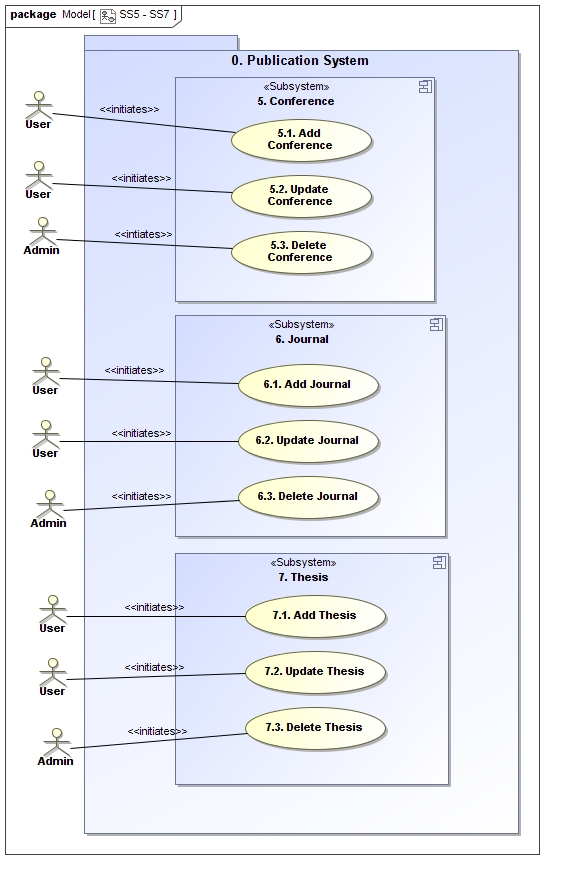
\includegraphics[width=\textwidth]{SS5-SS7}
					\caption{Use case diagram for the Conference, Journal and Thesis Subsystems}
				\end{figure}
		\subsection{Required Functionality}
			\subsubsection{User Subsystem Use Case}
				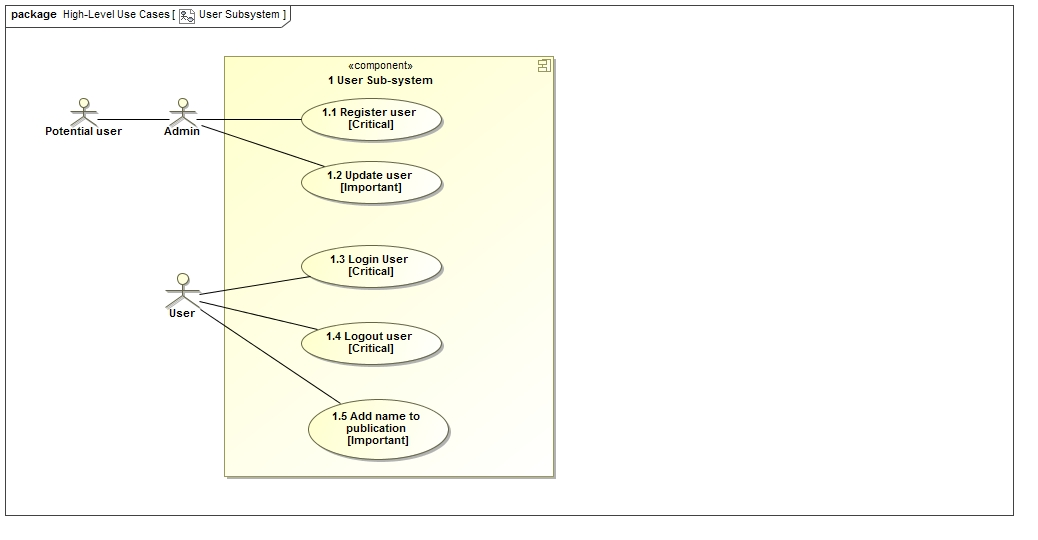
\includegraphics[width=\textwidth]{UserSubsystem}
				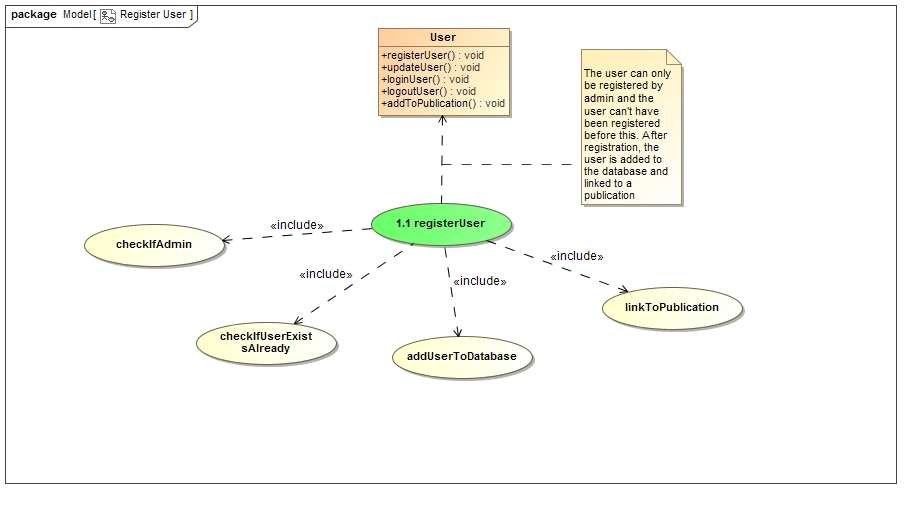
\includegraphics[width=\textwidth]{RegisterUser}
				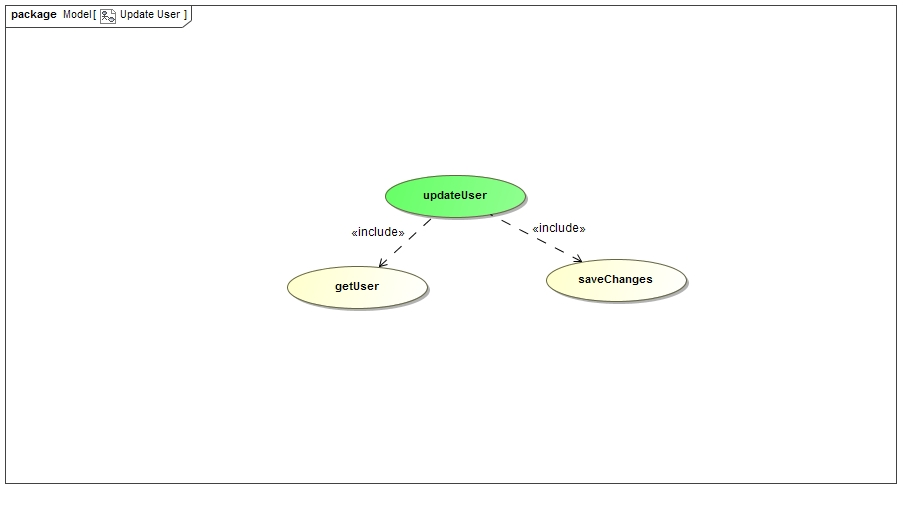
\includegraphics[width=\textwidth]{UpdateUser}
				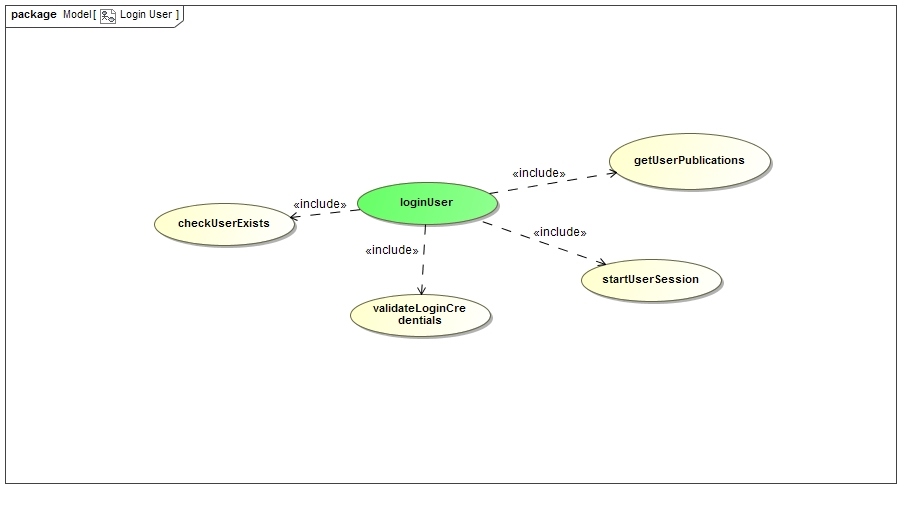
\includegraphics[width=\textwidth]{LoginUser}
				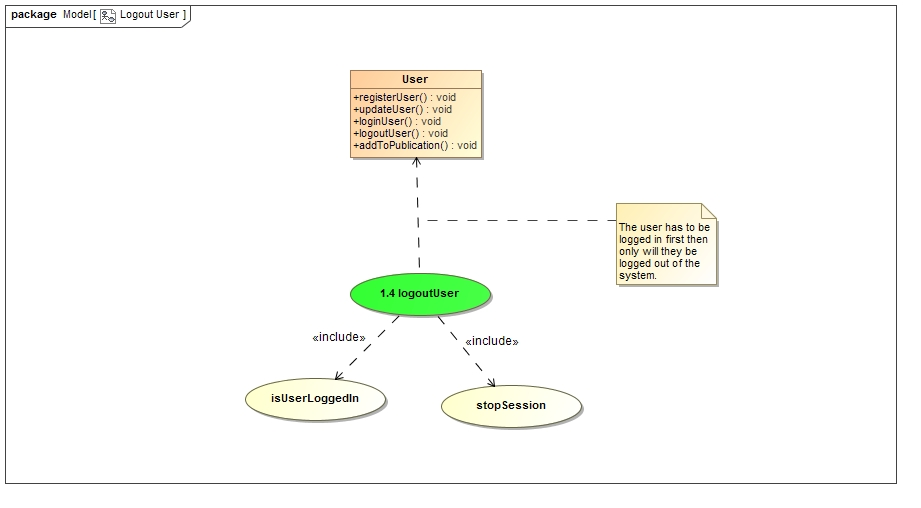
\includegraphics[width=\textwidth]{LogoutUser}
				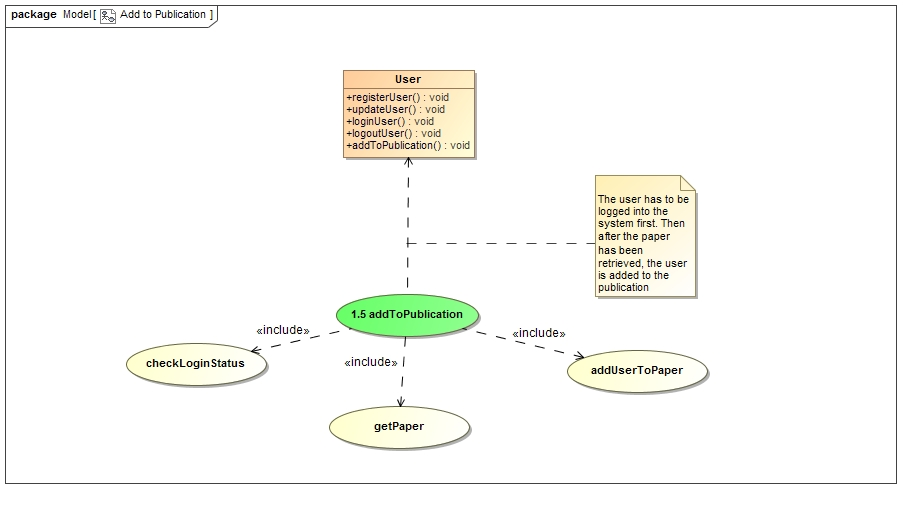
\includegraphics[width=\textwidth]{AddtoPublication}
			\subsubsection{Research Group Subsystem Use Case}
				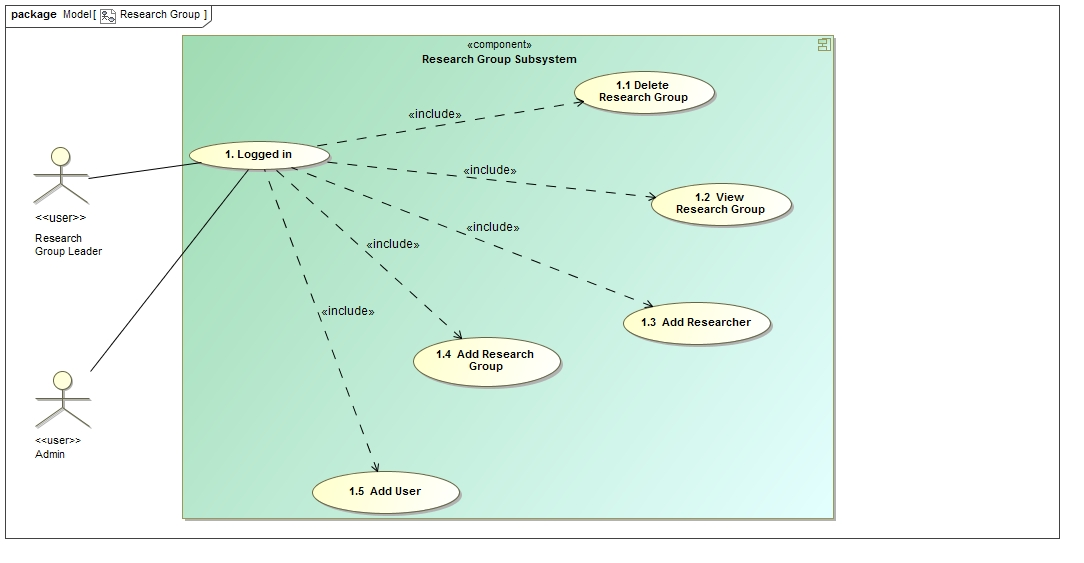
\includegraphics[width=\textwidth]{ResearchGroup}
			\subsubsection{Conference Subsystem Use Case}
				\begin{figure}
					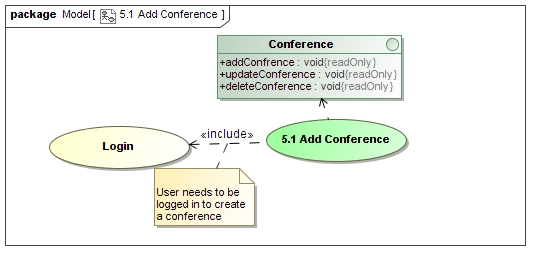
\includegraphics[width=\textwidth]{5.3-SS5-7/Add-Conference}
					\caption{Add Conference}
				\end{figure}
				\begin{figure}
					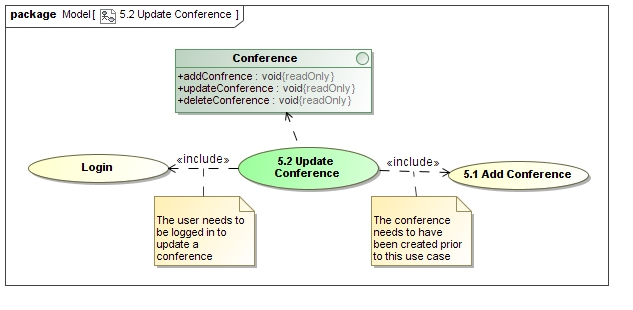
\includegraphics[width=\textwidth]{5.3-SS5-7/Update-Conference}
					\caption{Update Conference}
				\end{figure}
				\begin{figure}
					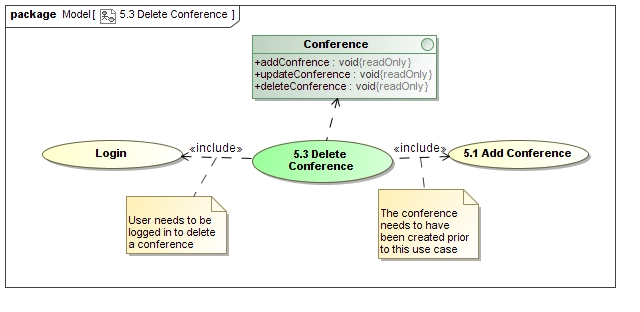
\includegraphics[width=\textwidth]{5.3-SS5-7/Delete-Conference}
					\caption{Delete Conference}
				\end{figure}
			\subsubsection{Journal Subsystem Use Case}
				\begin{figure}
					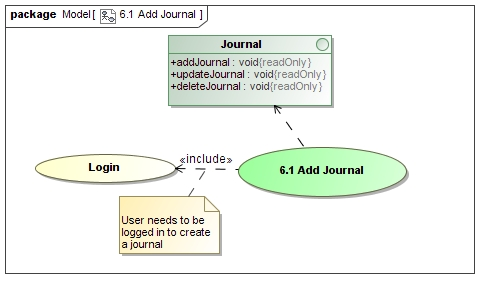
\includegraphics[width=\textwidth]{5.3-SS5-7/Add-Journal}
					\caption{Add Journal}
				\end{figure}
				\begin{figure}
					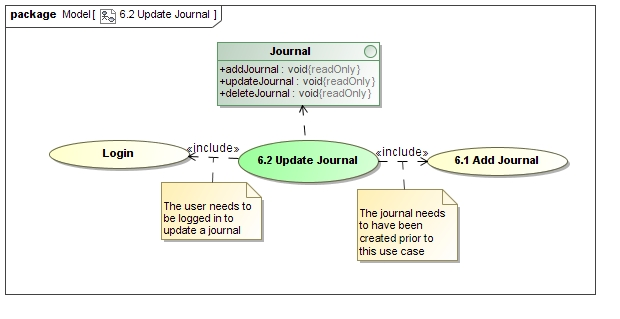
\includegraphics[width=\textwidth]{5.3-SS5-7/Update-Journal}
					\caption{Update Journal}
				\end{figure}
				\begin{figure}
					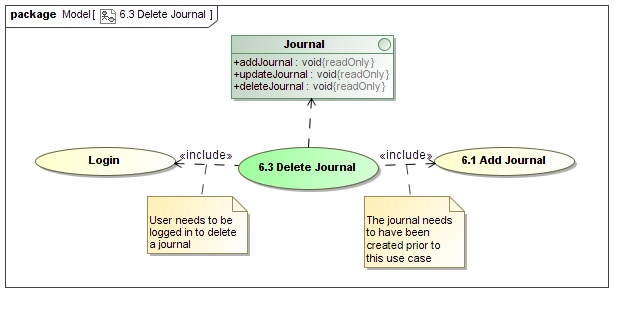
\includegraphics[width=\textwidth]{5.3-SS5-7/Delete-Journal}
					\caption{Delete Journal}
				\end{figure}
			\subsubsection{Thesis Subsystem Use Case}
				\begin{figure}
					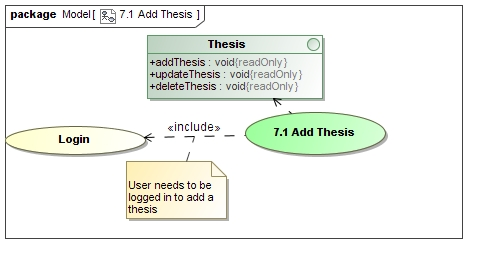
\includegraphics[width=\textwidth]{5.3-SS5-7/Add-Thesis}
					\caption{Add Thesis}
				\end{figure}
				\begin{figure}
					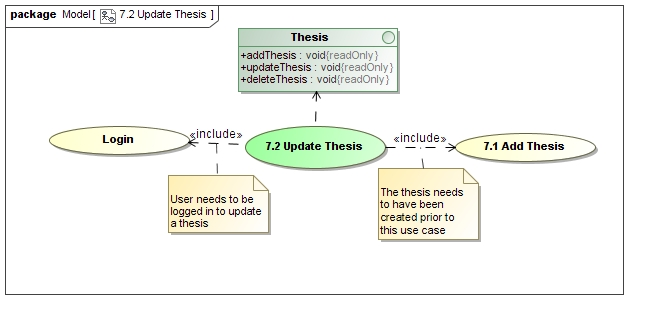
\includegraphics[width=\textwidth]{5.3-SS5-7/Update-Thesis}
					\caption{Update Thesis}
				\end{figure}
				\begin{figure}
					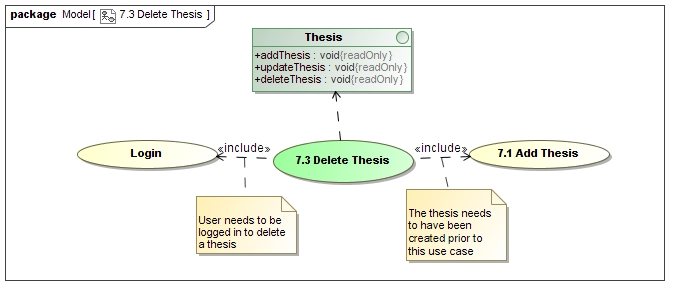
\includegraphics[width=\textwidth]{5.3-SS5-7/Delete-Thesis}
					\caption{Delete Thesis}
				\end{figure}
			\subsubsection{Report Subsystem Use Case}
				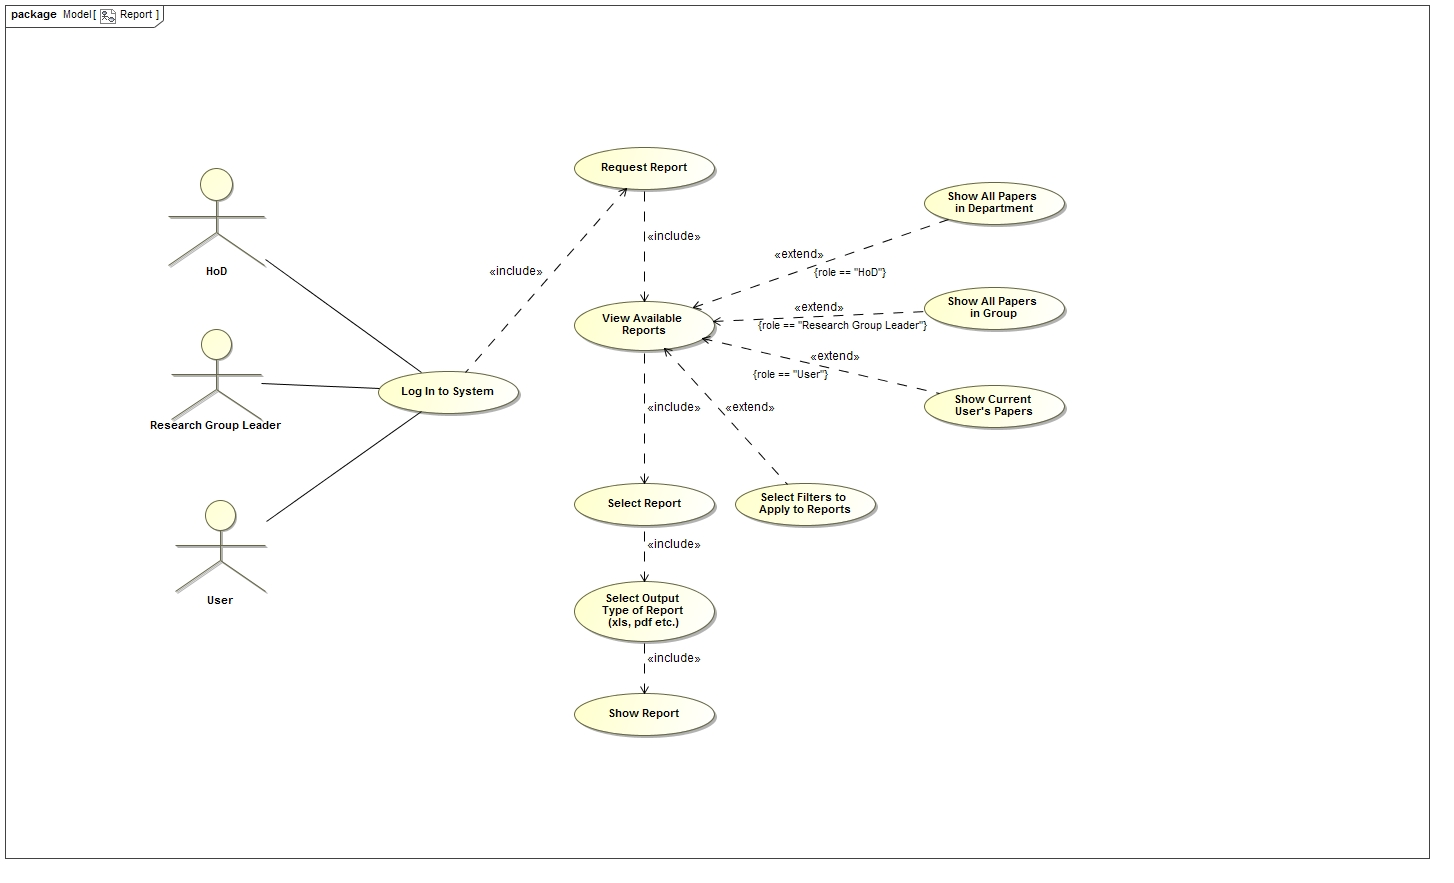
\includegraphics[width=\textwidth]{ReportUseCase}
		\subsection{Process Specifications}
			\subsubsection{Conference Subsystem}
				\begin{figure}
					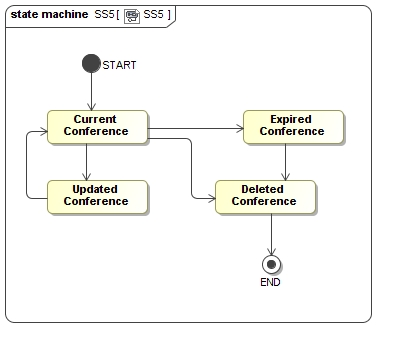
\includegraphics[width=\textwidth]{5.4-SS5-7/SS5}
					\caption{Conference State Diagram}
				\end{figure}
			\subsubsection{Journal Subsystem}
				\begin{figure}
					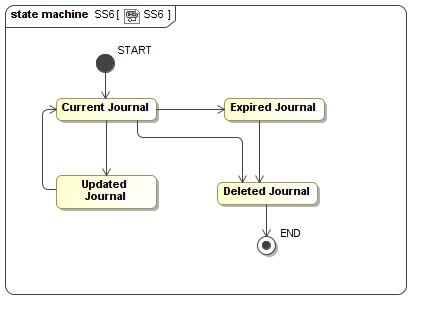
\includegraphics[width=\textwidth]{5.4-SS5-7/SS6}
					\caption{Journal State Diagram}
				\end{figure}
			\subsubsection{Thesis Subsystem}
				\begin{figure}
					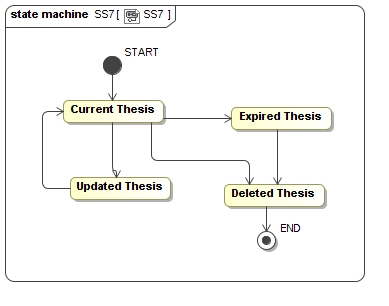
\includegraphics[width=\textwidth]{5.4-SS5-7/SS7}
					\caption{Thesis State Diagram}
				\end{figure}
		\subsection{Domain Model}
			\begin{figure}
					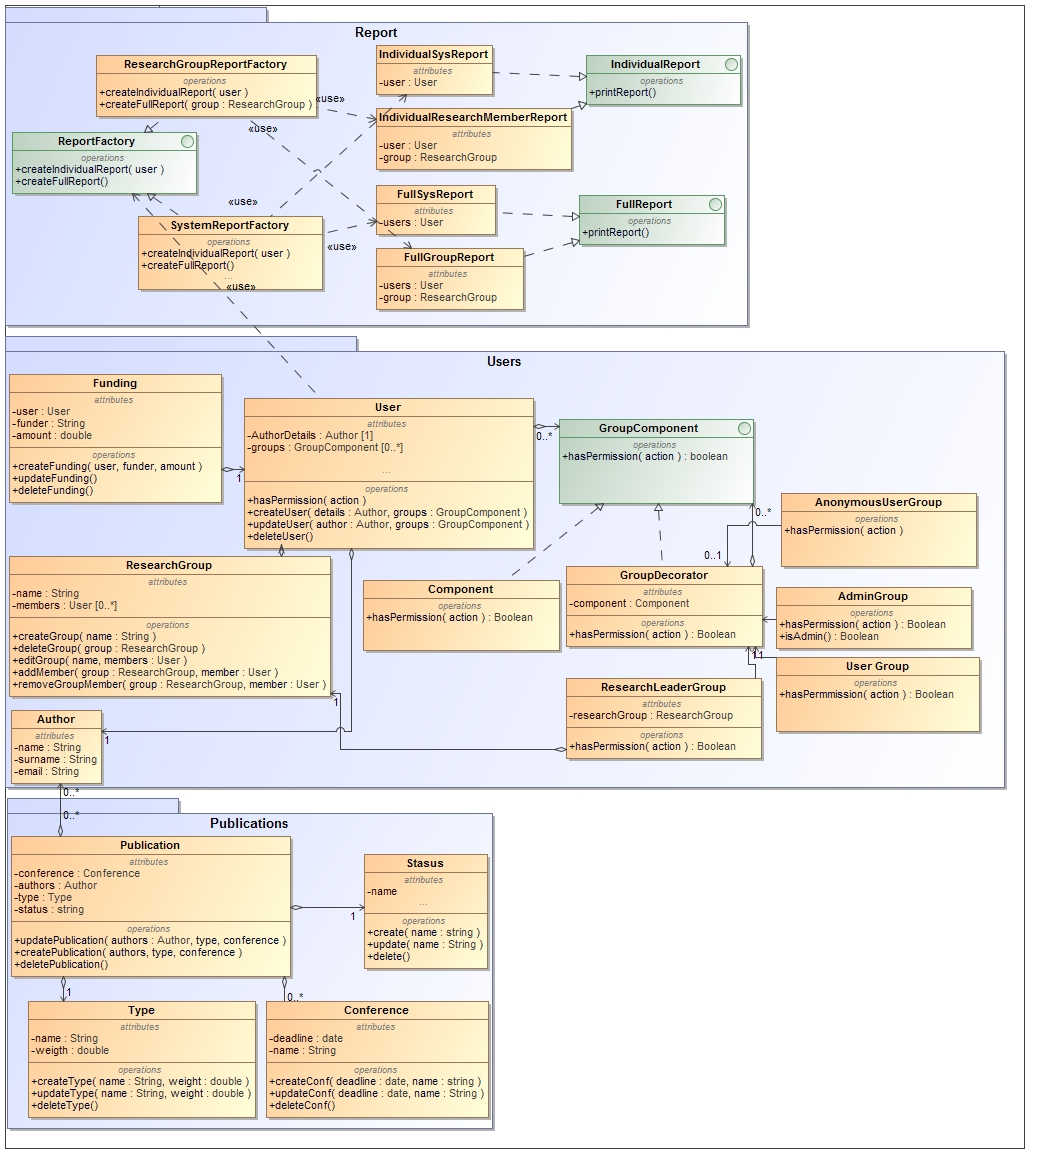
\includegraphics[width=\textwidth]{DomainModel/DomainModel}
					\caption{Domain Model}
			\end{figure}
	\section{Open Issues}
	\begin{itemize}
		\item What does DoE stand for?
		\item Specifics with regard to the DoE and UP weighted contributions
		\item Researcher funding
	\end{itemize}

\end{document}
